\section{Latency for DC conversations}

\subsection{Methodology}
Bearing in mind that the primary goal for this part is to understand the partition of latency from end-users' perspective, we designed the experiment to perform data center related tasks. We expect the model in Fig.\,\ref{fig:DC_model} to be used, and the fractions in the WAN and the DC are also shown. 

\begin{figure}
  \centering
  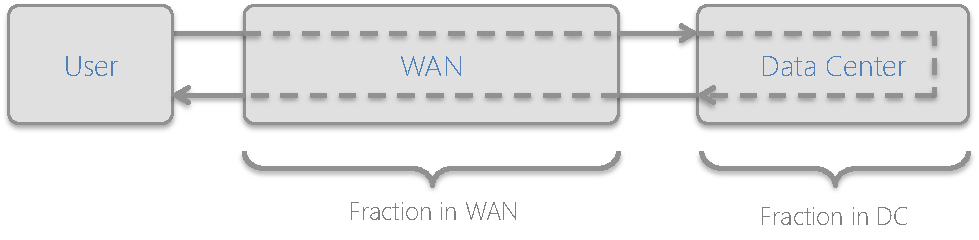
\includegraphics[width=\linewidth]{../figs/DC_model.pdf}
  \caption{Typical user-DC communication pattern}
  \label{fig:DC_model}
\end{figure}

As an representative user-facing service, we have chosen Google Search as the case study. One of the reason of choosing Google Search is that they provide an estimated time spent within their DC (Fig.\,\ref{fig:google_time}). From our analysis in Sec.\,\ref{sec:analysis}, this data is fairly accurate in reflecting the fraction in DC. 

\begin{figure}[t]
  \centering
  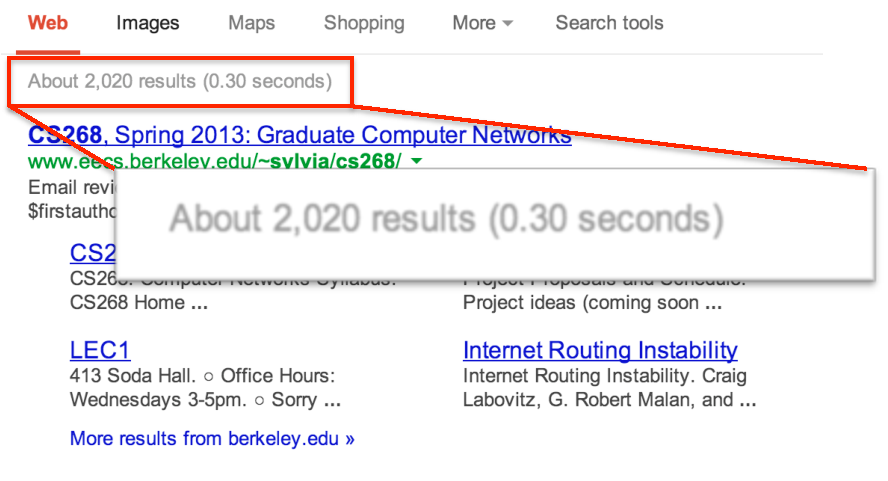
\includegraphics[width=0.85\linewidth]{../figs/GoogleTime.pdf}
  \caption{Google Search estimated time spent within Google in the return webpage}
  \label{fig:google_time}
\end{figure}

To measure the time for a single query, this can be easily done at the end-host side by timestamping the start and end of each query. But what to query remains a problem. Initially, we were suspecting that caching might happens at the Internet-facing router in DC. Querying the hottest words which are likely to be cached might reveal the WAN fraction. On the other side, to force the query to be processed by the DC (eliminating caching), we use random string for search. The hottest words can be found in Google Trends\footnote{http://www.google.com/trends/hottrends}, and we generate random strings comprised of lower cases, upper cases and numbers with length 32. Though the analysis in Sec.\,\ref{sec:analysis} shows a different results instead of what we have expected. This methodology is still useful to understand the problem we are initially planning to solve. 

In the meantime, {\it ping} is performed to measure the networking latency from the user to Google. Since we plan to conduct this experiment in geographically distributed fashion, and Google has many user-facing servers/IPs, we have to make sure we are measuring the right one. In this case, in additional to application layer HTTP conversation, we use {\it tcpdump} to capture all the packets and find out Google's IP address to ping.
 
In summary, to conduct the WAN vs. DC measurement, we issue query to Google and measure four different ``times'', shown in Table.\,\ref{tab:DC_method}.

\begin{table}
  \begin{tabular}{p{2.8cm} | p{5cm}}
    \hline
    type & description \\
    \hline
    Hot-trend-query time & the time spent to query a hot trend word to Google. \\
    Random-query time & the time spent to query a 32-character random string.  \\
    Ping time & the networking layer round-trip time to the responded Google IP address. \\
    Google time & Google's estimated time spent within their DC. \\
    \hline
  \end{tabular}
  \caption{Four different ``times'' measured}
  \label{tab:DC_method}
\end{table}


% \begin{itemize}
% \setlength{\leftmargin}{-1pt}
% \setlength{\itemsep}{1pt}
% \setlength{\parskip}{0pt}
% \setlength{\parsep}{0pt}
% \item Hot-trend-query time \\
%   the time spent to query a hot trend word to Google. 
% \item Random-query time -- the time spent to query a 32-character random string. 
% \item Ping time -- the networking layer round-trip time to the responded Google IP address.
% \item Google time -- Google's estimated time spent within their DC.
% \end{itemize}


\subsection{Implementation and Experiement}
\label{sec:impl-exper}


We implement this measurement script in Python, and use {\it cron} to schedule the execution every two hours. Each time, the script will first visit Google Trends webpage and obtain the hot-trend words for that hour. Together with random generated strings, we obtain a list of 20 words for query. 
The entire list is queried for 10 times repeatedly, and four ``times'' are recorded. Each query is conducted using Python urllib2 library through HTTP, and the query address is \url{http://www.google.com/search?hl=en\&output=search\&q=query}.\footnote{One thing to notice about our implementation is that it's actually not allowed to send automated query to Google according to their Terms of Service. And if Google detects it, they will show the following message: ``Our systems have detected unusual traffic from your computer network.'', and the users will be required to enter an CAPTCHA. One possible workaround is to limit the query speed. So after each query, we delayed the script for 5 seconds. We should point out that there are at most $12\times20$ queries per day, which is small.}

While doing the query, we use {\it tcpdump} to monitor the incoming and outgoing traffic on port 80. By inspecting the TCP traces, we can find the specific Google IP that responds our query, and we then {\it ping} it for 10 times.  {\it tcpdump} and {\it ping} are done using Python subprocess module.


\subsection{Analysis}
\label{sec:analysis}

Present the results and describe what we learned from the data.
Consider putting an appendix of all planetlab nodes we have used.

\begin{figure*}[!htb]
  \centering
  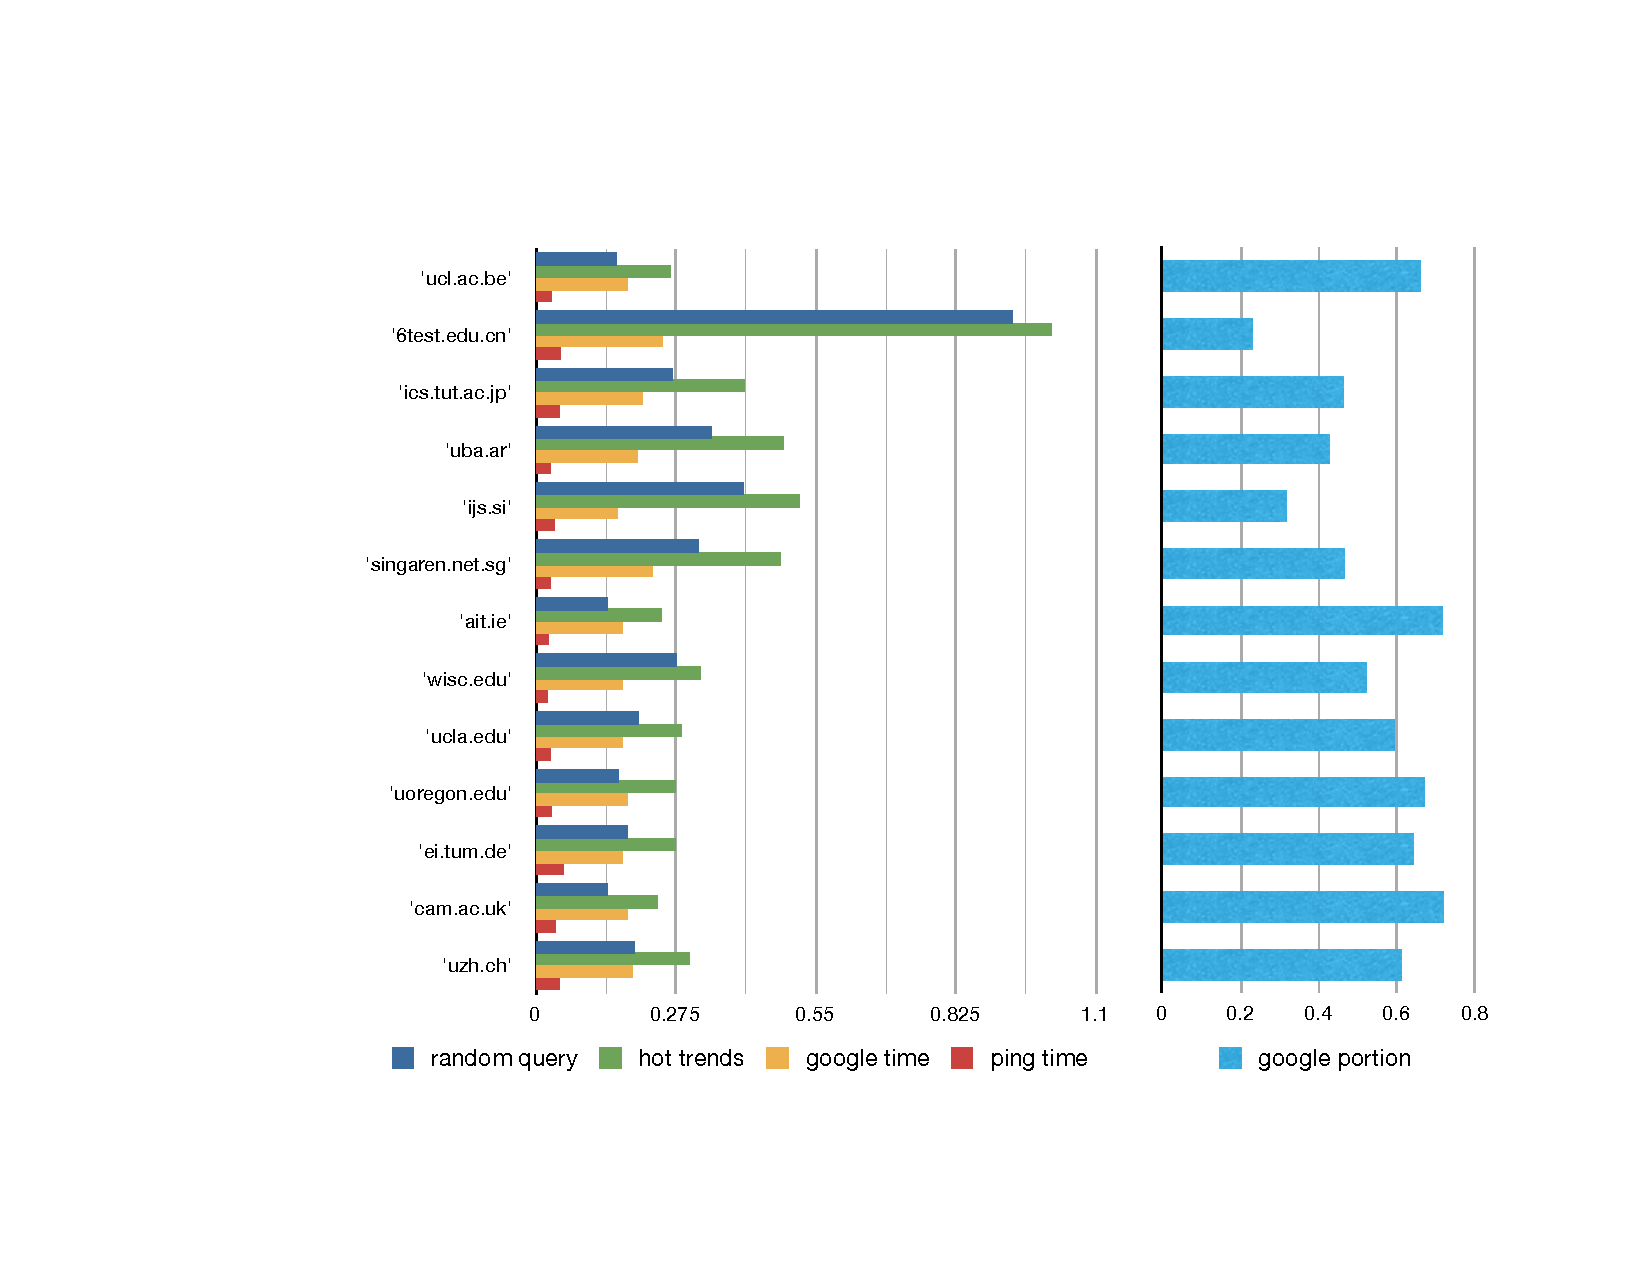
\includegraphics[width=\linewidth]{../figs/data_center.pdf}
  \caption{The latency measured in DC conversation experiments}
  \label{fig:data_center}
\end{figure*}


%%% Local Variables: 
%%% mode: latex
%%% TeX-master: "main"
%%% End: 

